\chapter{Metodología}

La metodología que se ha usado para llevar a cabo el proyecto se basa en las \textbf{metodologías ágiles} como \textbf{Scrum}.

 \vspace{0.5cm}

Este tipo de metogologías suelen aplicarse en \textbf{proyectos que se realizan en grupo} para así separar bien las tareas, que todos los integrantes puedan trabajar desacopladamente e ir obteniendo resultados lo antes posible. No obstante, este proyecto se trata de un trabajo que se va a realizar únicamente por una persona, pero aún así sigue siendo una buena idea aplicar este tipo de metodologías ya que este es un proyecto donde queremos \textbf{tener un producto lo antes posible}, y que nos permita ir mejorándolo, añadiéndole funcionalidades o características extras que lo mejoren. 

 \vspace{0.5cm}

Así pues, se ha \textbf{adaptado} la metodología Scrum al desarrollo de este videojuego para NDS aplicando un \textbf{desarrollo iterativo}. Al principio, se planificó  una serie de iteraciones teniendo en cuenta el tiempo disponible, asignándoles los objetivos o tareas generales que se debían realizar en éstas. A pesar de que en las metodologías ágiles las iteraciones son de periodos cortos de tiempo, en este caso se decidió ampliar esos tiempos ya que el equipo de trabajo es de únicamente una persona. No obstante las iteraciones se planeó que duraran como máximo un mes.

 \vspace{0.5cm}

Por otro lado, después de cada iteración, se extraía una \textbf{conclusión} del trabajo desarrollado en ésta y se valoraba \textbf{modificar la planificación inicial} si surgía algún problema.

 \vspace{1cm}

\section{Planificación}

A continuación se detallan las iteraciones que se establecieron, con las tareas que se iban a realizar en estas:

\subsection{Iteración 0}

\begin{itemize}
 \item Documentarse sobre cómo desarrollar para NDS. 
 \item Realizar pruebas de dibujado simples que nos den una práctica y conocimiento necesarios para empezar a crear el proyecto.
 \item Analizar los referentes y realizar un diseño del juego.
\end{itemize}

\subsection{Iteración 1 - 4}

\begin{itemize}
 \item Desarrollo del juego, de sus mecánicas y algoritmos necesarios.
 \end{itemize}
 
 \subsection{Iteración 5 - 6}
 
 \begin{itemize}
 \item Mejoras visuales y de retroalimentación para el usuario. 
 \item Realización de pruebas para encontrar fallos tanto en el funcionamiento como en el diseño.

 \end{itemize}
 
  \vspace{0.5cm}
 
 Por último, para llevar un \textbf{seguimiento de la planificación} se ha utilizado la herramienta \textbf{Trello}. Se creó un tablero con la listas de tareas generales para especificar las tareas que el proyecto requería, la lista de iteración actual, para especificar qué tareas se debían realizar en esa iteración, la lista WIP\footnote{WIP: del inglés, \textit{Work In Progress}.}, que contiene las tareas en las que se están trabajando actualmente, y la lista finalizado, que contiene las que ya se han acabado. Además también tiene una lista de problemas, para ir apuntando los inconvenientes que surjan durante el desarrollo y asegurar así que no se quedaban sin resolver.
 
  \vspace{0.5cm}
 
 Se trata de una herramienta muy cómoda, pues de un simple vistazo puedes saber el estado del proyecto, y, además, es muy cómoda de utilizar.

  \vspace{0.5cm}
  
  \begin{figure}[htbp]
\centering
  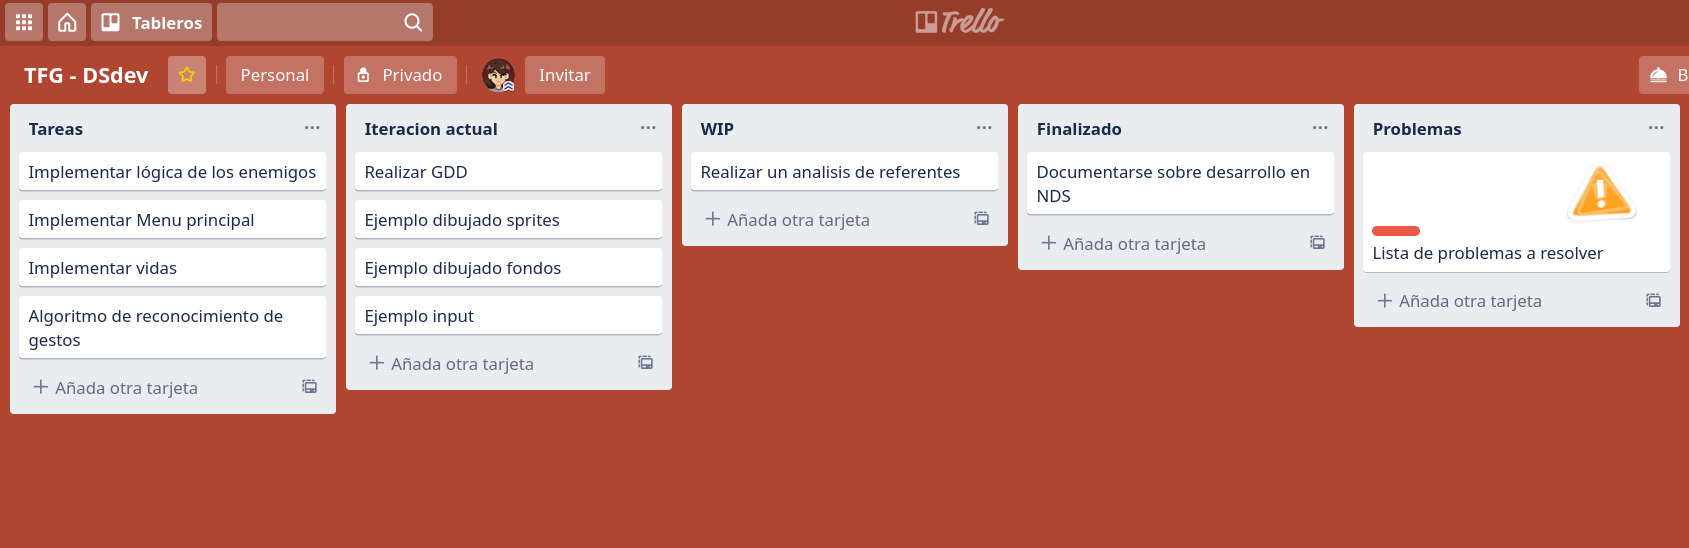
\includegraphics[width=1\textwidth]{archivos/trello.png}
  \caption{Estado del tablero de Trello durante la iteración 0.}
  \label{fig:trello}
\end{figure}

 
\section{Mínimo producto viable}

El diseño realizado en el apartado Diseño del juego está pensado para que, en el mejor de los casos se puedan implementar todas las mecánicas, tipos de enemigos, pantallas, etc. en el tiempo disponible de desarrollo, sin embargo, es poco probable que así sea.

\vspace{0.5cm}

Surgirán problemas, tanto externos como internos, de eso no cabe duda, y no queremos vernos en la situación de estar a pocas semanas de la fecha final y \textbf{solo tener un prototipo}. Es por ello que hay que estar preparado para ese problema y definir una versión simplificada, que siga funcionando como juego y sea un \textbf{producto cerrado} de principio a fin, algo que la gente pueda probar para ver si le gustan las mecánicas o no y a partir de ahí \textbf{trabajar iterativamente} sobre ello añadiéndole las funcionalidades explicadas anteriormente con un \textbf{orden de prioridad}.

\vspace{0.5cm}

Así pues, el mínimo producto que se plantea es el siguiente:

\vspace{0.5cm}

Tendrá un \textbf{único y primer nivel}, donde los enemigos que aparezcan solo tengan \textbf{un patrón} que será al azar entre \textbf{dos tipos distintos} (horizontal y vertical).

\vspace{0.5cm}

Se implementará la \textbf{muerte} del jugador, así como la \textbf{victoria}, de modo que el juego pueda \textbf{rejugarse} tantas veces como se quiera. No obstante, no sería necesario implementar aún las respectivas pantallas de fin de juego y victoria, con volver a la pantalla principal bastaría.

\vspace{0.5cm}

Por último carecería de animaciones y sonido, pues implementar las \textbf{mecánicas} es \textbf{prioritario} frente a perfeccionar lo visual. Sin embargo, sí que se implementará el dibujado del \textbf{rastro del lápiz en la pantalla táctil}, así nos servirá como \textbf{método de depurado} en caso de que el reconocimiento de gestos nos de problemas.

\vspace{0.5cm}

En la siguiente imágen se muestra un mockup de lo que sería el mínimo producto viable:

\vspace{0.5cm}

\begin{figure}[htbp]
\centering
  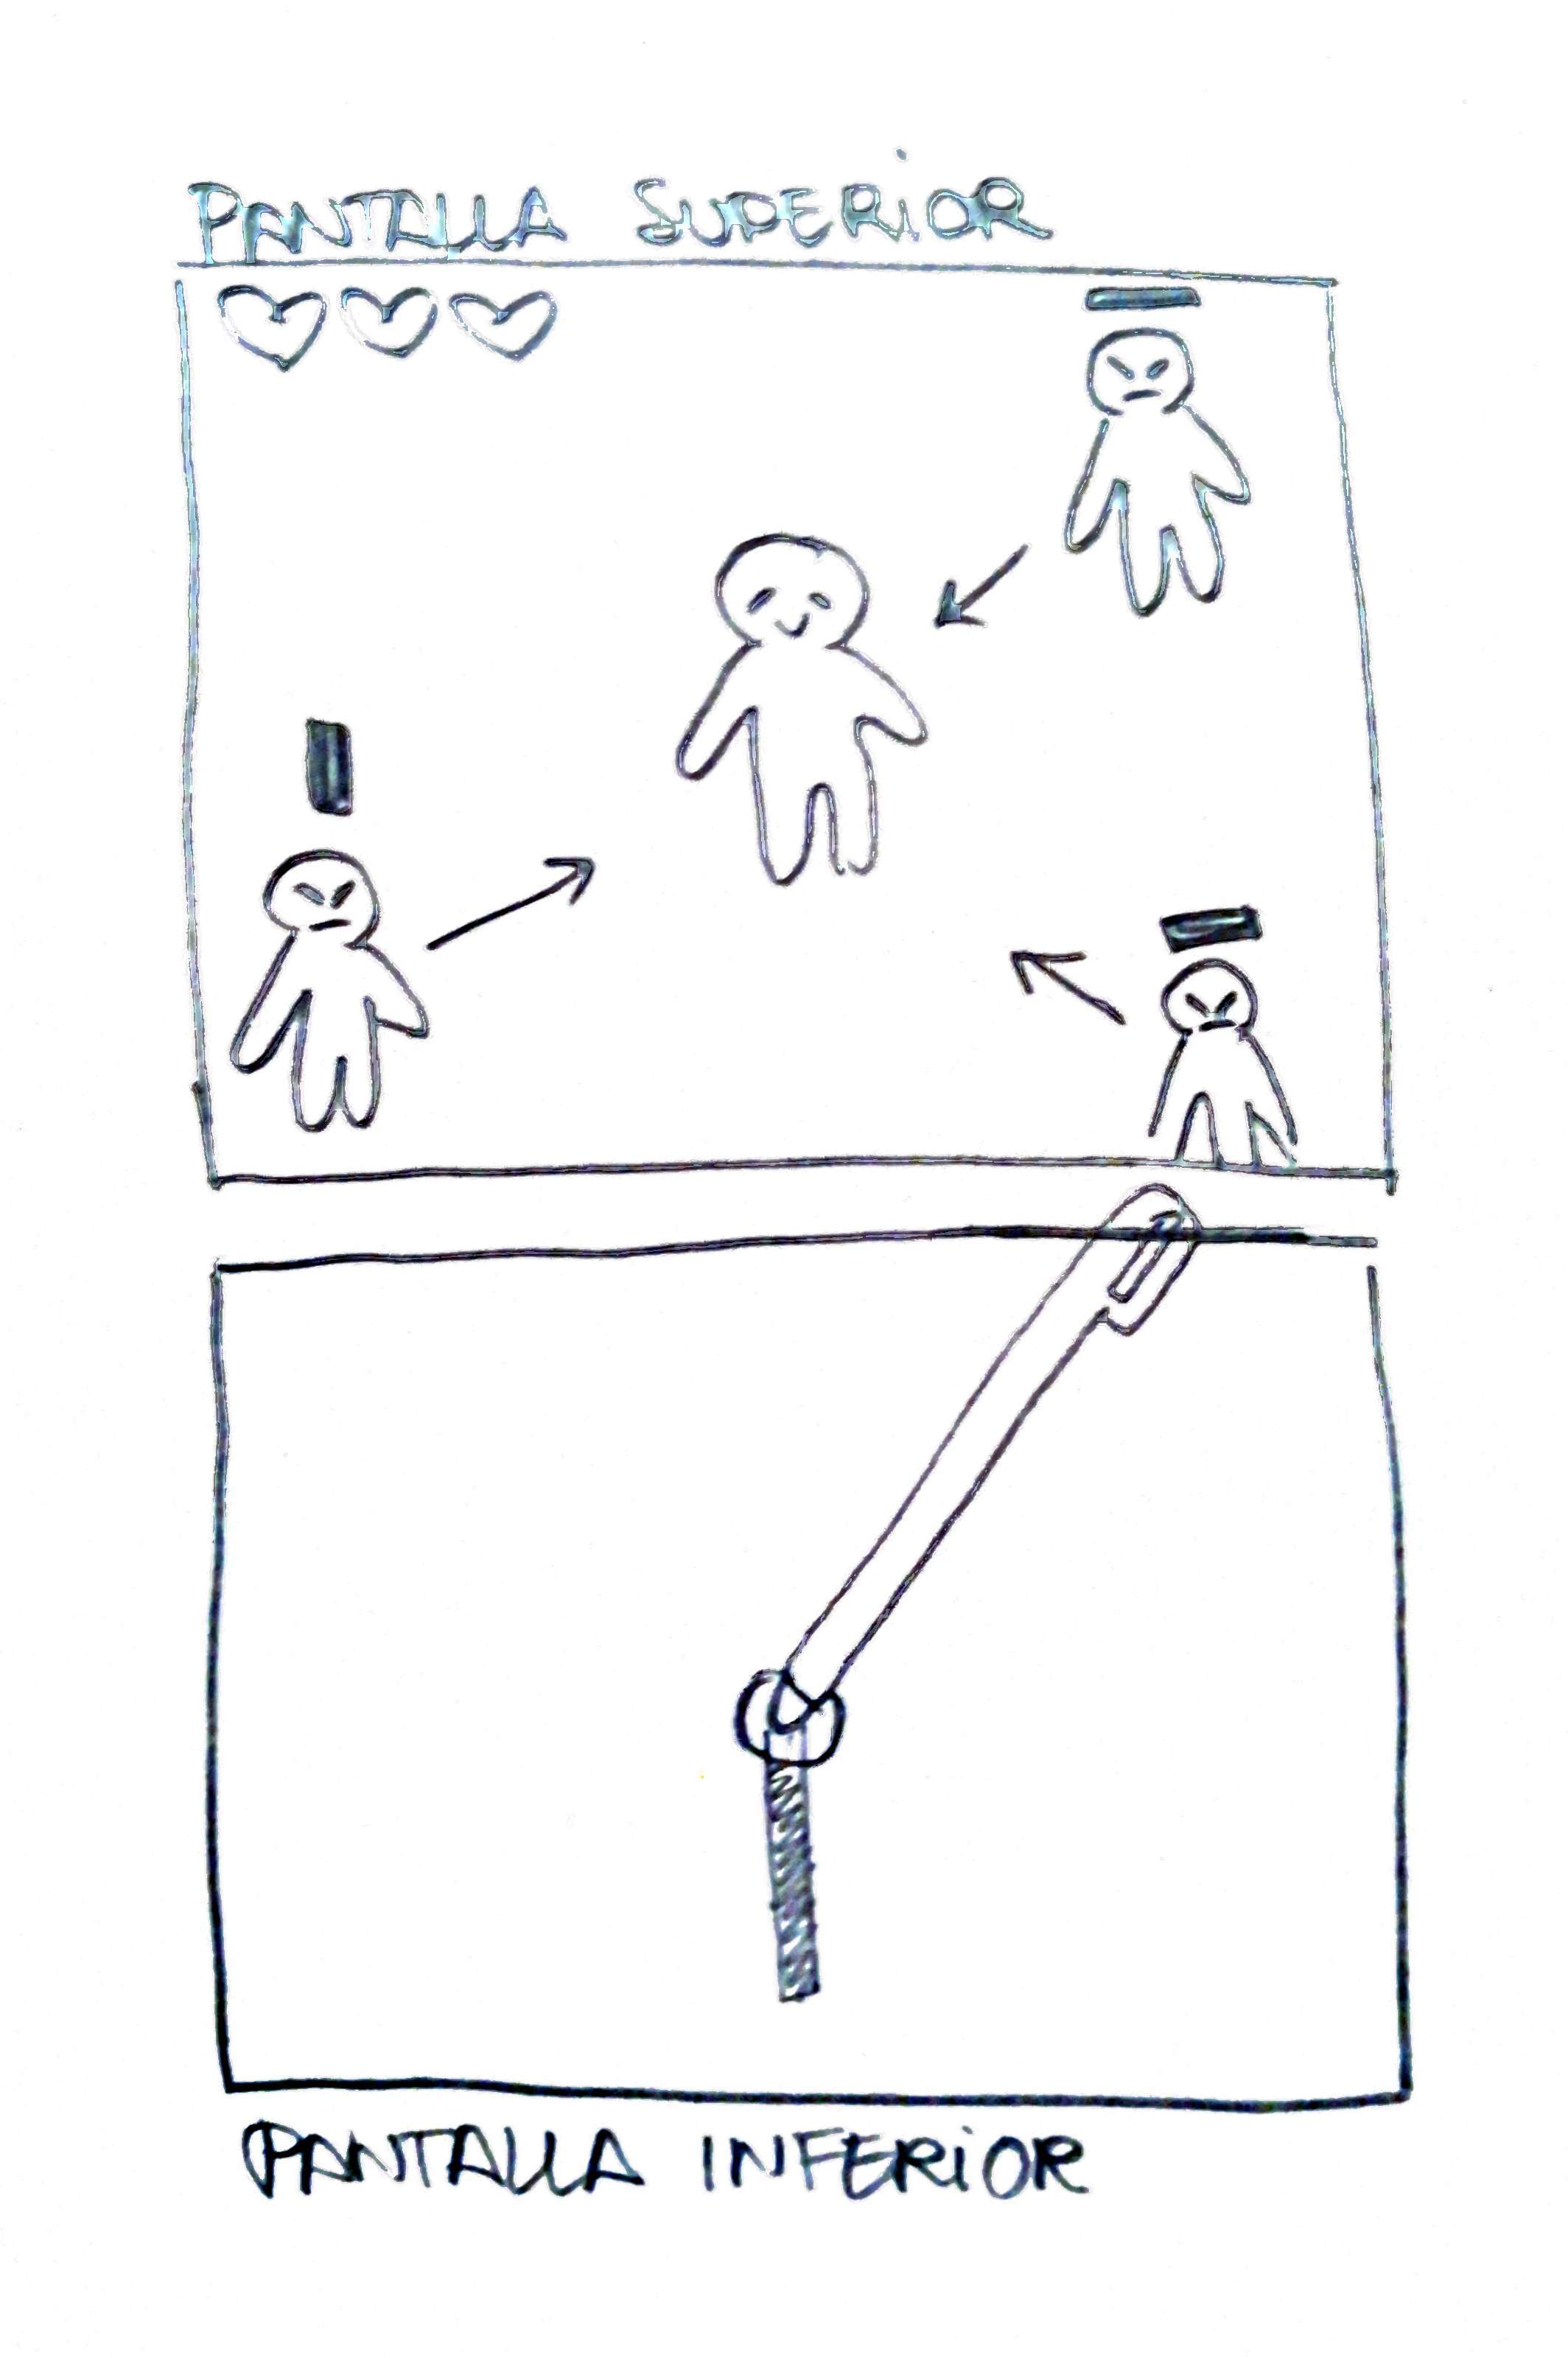
\includegraphics[width=0.4\textwidth]{archivos/minimoprod.jpg}
  \caption{Concepto del mínimo producto viable.}
  \label{fig:minimoprod}
\end{figure}
